\documentclass[12pt,a4paper]{article}
\usepackage[utf8]{inputenc}
\usepackage{geometry}
\usepackage{tabularx}
\usepackage{hyperref}
\usepackage{graphicx} % Resim eklemek için
\usepackage{float}    % Resim konumlarını sabitlemek için (H)
\geometry{a4paper, margin=1in}

\title{\textbf{CSE344 - System Programming} \\ \Large Homework \#2 Report}
\author{Muhammed Korkmaz \\ Student ID: 220104004043}
\date{\today}

\begin{document}
\maketitle

\section{Introduction}
This report outlines the design and implementation of an advanced, multi-process POSIX-compatible file search utility. The primary objective of this program is to recursively traverse a specified directory subtree using a parent-worker process model. The utility distributes the search workload among multiple worker processes, filtering files based on a custom regular expression pattern and an optional minimum size constraint. The parent process safely collects the results via signals and inter-process communication, ultimately displaying a well-formatted hierarchical tree and an execution summary.

\section{Program Design and Process Management}
To effectively manage the workload and strictly prevent buffer overflow issues, a robust Parent-Worker architecture was designed.

\begin{itemize}
    \item \textbf{Directory Partitioning:} The parent process dynamically reads the immediate subdirectories of the target root directory. These subdirectories are then partitioned and assigned to the worker processes in a round-robin fashion. If the root directory contains files directly under it, they are exclusively searched by the parent process to ensure no files are overlooked.
    \item \textbf{Inter-Process Communication (IPC):} Instead of using anonymous pipes, which can suffer from buffer limitations during massive directory traversals, temporary files were utilized. Each worker writes its matched paths and scanned file count to a unique \texttt{worker\_<PID>.txt} file. The parent reads these files during the summary phase and safely removes them.
    \item \textbf{Memory Management:} To handle exceptionally large directory structures (such as \texttt{/usr/share/doc}) without encountering Segmentation Faults, static arrays for subdirectory tracking were replaced with dynamically managed memory using \texttt{malloc()} and \texttt{realloc()}. All allocated memory is rigorously freed before termination to prevent memory leaks.
\end{itemize}

\section{Signal Handling and Synchronization}
Strict adherence to async-signal-safety was maintained throughout the implementation. All signal handlers utilize \texttt{volatile sig\_atomic\_t} flags, completely avoiding unsafe functions like \texttt{printf()} within the handler context.

\begin{enumerate}
    \item \textbf{SIGUSR1 \& SIGCHLD:} Upon task completion, workers send a \texttt{SIGUSR1} signal to the parent. The parent captures the sender's PID using the \texttt{SA\_SIGINFO} flag. A \texttt{SIGCHLD} handler using \texttt{waitpid()} with \texttt{WNOHANG} is implemented to reap terminated children instantly, strictly preventing zombie processes.
    \item \textbf{SIGINT \& SIGTERM:} If the user triggers an interrupt (CTRL-C), the parent catches \texttt{SIGINT}, sends \texttt{SIGTERM} to all active workers, and waits for a brief period. Workers catch \texttt{SIGTERM}, print their partial match counts, and exit cleanly. The parent then aggregates the partial results and terminates.
\end{enumerate}

\subsection{Preventing Advanced Signal Race Conditions}
A critical synchronization challenge (Lost Wakeup / Signal Merging) occurs when multiple workers finish their tasks in the exact same millisecond. The Linux kernel might merge simultaneous \texttt{SIGUSR1} signals, or a \texttt{SIGCHLD} might arrive before \texttt{SIGUSR1} is fully processed, causing false "unexpected termination" errors. 

To definitively solve this, a \textbf{Staggered Signal Emission} and \textbf{Signal Masking} technique was implemented. Workers calculate a brief delay using \texttt{usleep(worker\_index * 25000)} before emitting \texttt{SIGUSR1}, ensuring signals arrive sequentially. Furthermore, the parent uses \texttt{sigprocmask()} to block \texttt{SIGUSR1} and \texttt{SIGCHLD} before forking, protecting the PID registry array, and uses \texttt{sigsuspend()} to safely wait for signals without deadlocking. In addition, workers ignore \texttt{SIGINT} directly, leaving the signal catching entirely to the parent process.

\section{Pattern Matching Implementation}
As the use of external regular expression libraries was prohibited, a custom \texttt{match\_regex} function was implemented from scratch. The \texttt{+} operator correctly acts on the \textbf{immediately preceding character} on its left side, as per standard regex conventions.

The algorithm uses a recursive substring matching approach. When a \texttt{+} is detected at the next index in the pattern, the function creates two branches of recursion: one that consumes the matching character and stays on the \texttt{+} to consume more, and another that moves past the \texttt{+}. The comparison is case-insensitive, accomplished by converting both characters to lowercase via \texttt{tolower()} before comparison.

\section{System Calls and POSIX Functions Used}
The program exclusively relies on standard POSIX functions for process management, signal handling, and file operations.
\vspace{0.5cm}

\noindent
\begin{tabularx}{\textwidth}{|l|X|}
\hline
\textbf{Function} & \textbf{Purpose} \\
\hline
\texttt{fork()} & Creates child (worker) processes to distribute the directory traversal workload. \\
\hline
\texttt{waitpid()} & Reaps terminated child processes to prevent zombies and retrieves their exit statuses. \\
\hline
\texttt{sigaction()} & Safely installs signal handlers for \texttt{SIGINT}, \texttt{SIGTERM}, \texttt{SIGCHLD}, and \texttt{SIGUSR1}. \\
\hline
\texttt{sigprocmask()} & Blocks and unblocks signals to protect critical sections and prevent race conditions. \\
\hline
\texttt{sigsuspend()} & Safely puts the parent process to sleep until a specific unmasked signal arrives. \\
\hline
\texttt{opendir() / readdir()} & Opens and reads successive entries from directory streams. \\
\hline
\texttt{lstat()} & Retrieves file metadata (specifically size and type) for filtering criteria. \\
\hline
\end{tabularx}

\section{Error Handling}
Robust error handling is implemented across all system calls. If a worker encounters an inaccessible directory, it silently skips it to allow uninterrupted processing of valid branches. If a worker terminates unexpectedly (e.g., crashing before sending \texttt{SIGUSR1}), the parent's \texttt{SIGCHLD} handler detects the missing PID registration and logs a detailed warning to \texttt{stderr} without halting the entire program.

\newpage
\section{Test Scenarios and Screenshots}
Here are the executions of the mandatory test scenarios proving the stability, correctness, and safety of the implemented utility.

\subsection*{Directory Structure Initialization}
The directory structure was meticulously created to match the assignment requirements, containing 5 directories and 9 files.
\begin{figure}[H]
    \centering
    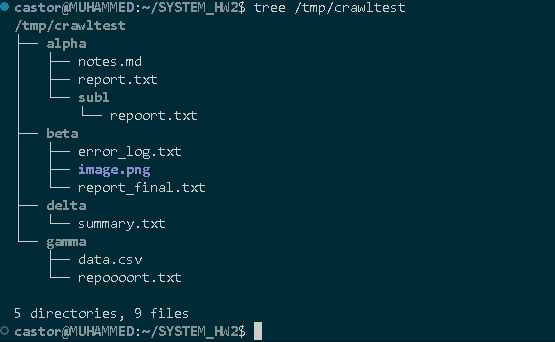
\includegraphics[width=0.7\textwidth]{tree.png}
    \caption{Initial directory structure verified using the \texttt{tree} command.}
\end{figure}

\subsection*{Test 1: Mandatory Search Scenario}
The program accurately builds the tree with correct hierarchical indentation and shows successful regex matching for the given pattern.
\begin{figure}[H]
    \centering
    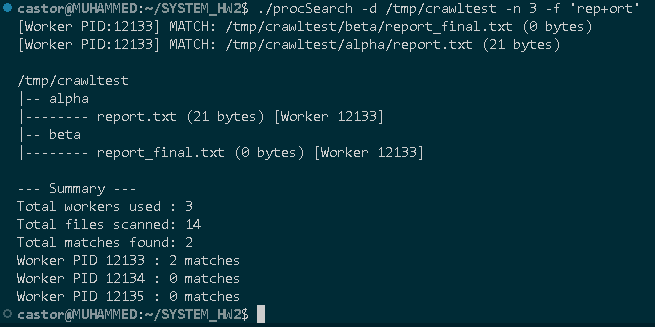
\includegraphics[width=\textwidth]{test1.png}
    \caption{Basic search tree and summary output.}
\end{figure}

\subsection*{Test 2: No Match Scenario}
Testing with a non-matching regex (\texttt{xyz+123}). The program does not crash and safely prints the "No matching files found" message with a 0-match summary.
\begin{figure}[H]
    \centering
    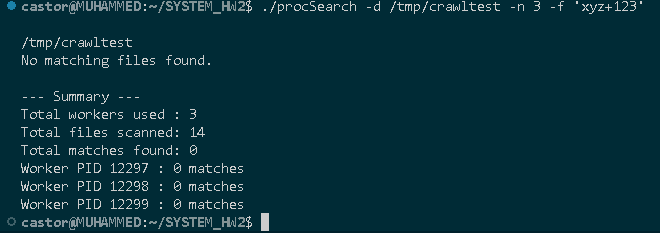
\includegraphics[width=\textwidth]{test2.png}
    \caption{Execution with no matching files.}
\end{figure}

\subsection*{Test 3: SIGINT (CTRL+C) and Zombie Process Check}
The program successfully catches the \texttt{SIGINT} signal during a massive directory scan, stops all workers safely, prints a partial summary, and leaves zero zombie processes behind.
\begin{figure}[H]
    \centering
    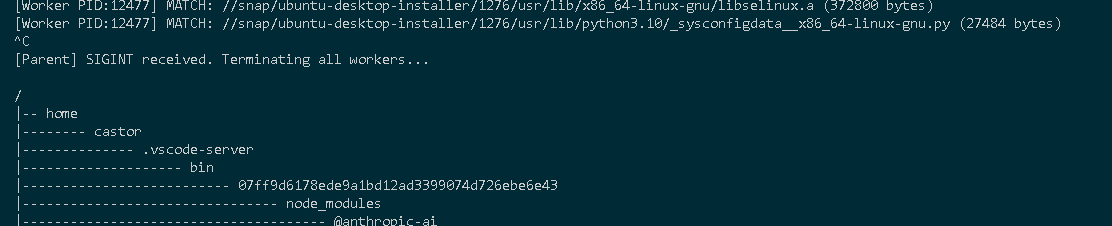
\includegraphics[width=\textwidth]{ctrlctest.png}
    \caption{Graceful shutdown initiated via CTRL+C.}
\end{figure}

\begin{figure}[H]
    \centering
    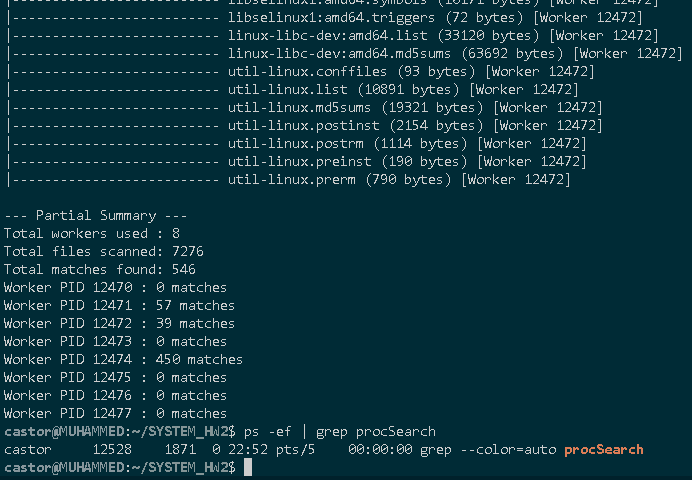
\includegraphics[width=\textwidth]{test3and4.png}
    \caption{Partial summary and process status verifying no zombie processes remain.}
\end{figure}

\section{Conclusion}
This implementation successfully fulfills all the requirements of an advanced multi-process file search utility. It accurately distributes workloads, manages complex IPC and signal race conditions, avoids deadlocks, and securely manages dynamic memory. The final output is presented in a clean, hierarchical tree format accompanied by a precise execution summary, demonstrating a deep understanding of Linux system programming concepts.

\end{document}